\begin{frame}{Le progrès de la science comme un processus \textit{discontinu}}
Le nouveau \textit{paradigme}\footnote{Découvertes scientifiques universellement reconnues.} est incompatible avec le précédent.
\begin{itemize}
\item \og{}rupture entre observation et expérimentation\fg{} 
{\footnotesize(\cite{bachelard1934formation})}
\item \og{}révolution scientifique\fg{} {\footnotesize(\cite{koyre1957closed})}
\item \og{}changement de paradigme\fg{} {\footnotesize(\cite{kuhn1962structure})} 
\end{itemize} 
\begin{figure}
    \centering
    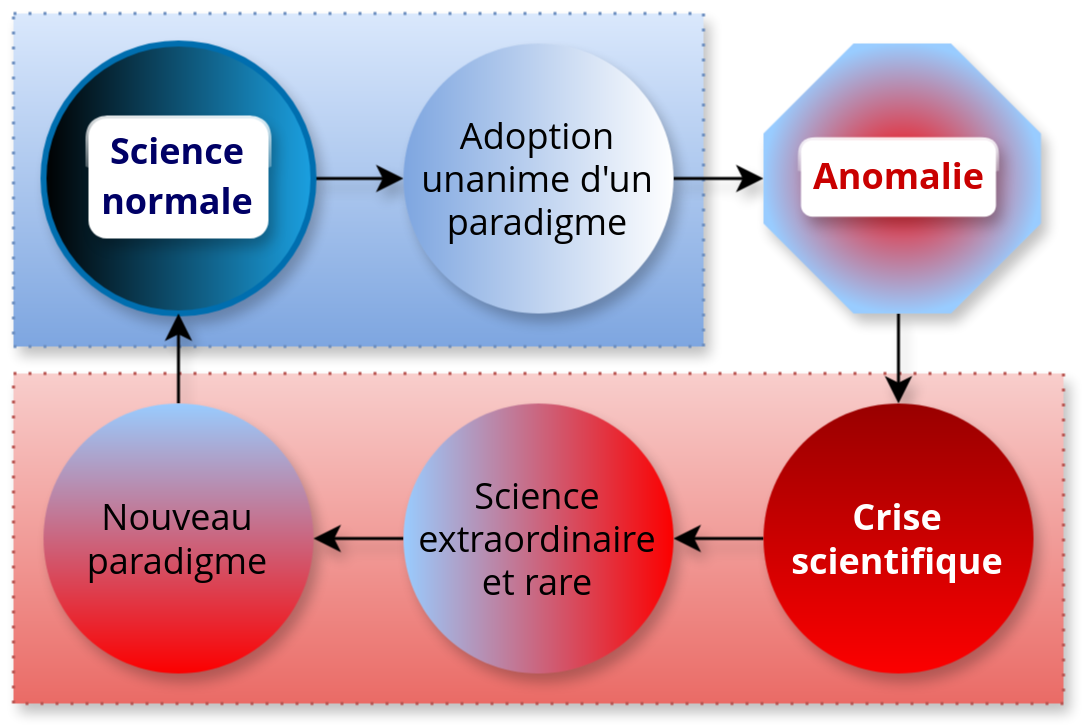
\includegraphics[width=65mm,scale=0.5]{pic/changement_paradigme.png}
    \caption{Conception kuhnienne du progrès scientifique, adaptée de {\scriptsize\textcite{amiri}}.}
    \label{fig:enter-label}
\end{figure}
\end{frame}
